%inizative bildverarbeitung
%llncs    article
\documentclass[a4paper,parskip=full-]{article}

\usepackage{amsmath}
\usepackage{amssymb}

\usepackage{subcaption}
\usepackage{float}
\restylefloat{figure}
\usepackage{graphicx}  % images
%\usepackage{qtree} % for trees
%auch für Bäume
%http://tex.stackexchange.com/questions/183866/tree-with-six-or-more-children
\usepackage{tikz, tikz-qtree}
\usepackage{pgfplots}
\usetikzlibrary{automata,topaths,plotmarks}
\usepackage{lmodern}  %THE tex font :)
\usepackage{url}  %urls in references
%\usepackage{prettyref}
%\usepackage{pstricks} %graphicv2
\usepackage{cite}
\usepackage{enumerate}
\usepackage{multicol}
\usepackage{xspace}

\usepackage{algorithmic} 
\usepackage{wasysym}
\usepackage[ngerman]{babel}
\usepackage[utf8]{inputenc} % Zeichenkodierung   utf8   latin1
%\include{biblio} % references
\usepackage{listings}                           % for source code inclusion
\usepackage{multirow} 
\usepackage{caption}
\usepackage{wrapfig}
\usepackage{color}

\usepackage{fancyvrb }

%absatz
\usepackage{setspace} 

%breaking math formulars automaticly
%http://tex.stackexchange.com/questions/3782/how-can-i-split-an-equation-over-two-lines
\usepackage{breqn}

%für kurze Enumarates wie i,I a, A etc.
\usepackage[shortlabels]{enumitem}

%Durchstreichungen
%\cancel
%http://de.wikibooks.org/wiki/LaTeX-Kompendium:_F%C3%BCr_Mathematiker#Durchstreichungen
\usepackage{cancel}

%Für Römische Zahlen
\usepackage{enumitem}
%\usepackage{romannum}%stdclsdv

%Durchstreicen möglich
\usepackage[normalem]{ulem}

%Bessere Brüche
\usepackage{nicefrac}

%bookmarks
%\usepackage[pdftex,bookmarks=true]{hyperref}
%[pdftex,bookmarks=true,bookmarksopen,bookmarksdepth=2]
\usepackage{hyperref}
%\usepackage{scrhack}

%fußnoten
\usepackage{footnote}
\usepackage{caption} 

\usepackage{geometry}
\geometry{verbose,a4paper,tmargin=25mm,bmargin=25mm,lmargin=15mm,rmargin=20mm}

%randnotiz
\newcommand\mpar[1]{\marginpar {\flushleft\sffamily\small #1}}
\setlength{\marginparwidth}{3cm}

%svg Grafiken
%http://tex.stackexchange.com/questions/122871/include-svg-images-with-the-svg-package
%\usepackage{svg}

\usepackage{pgf}

%http://tex.stackexchange.com/questions/48653/making-subsections-be-numbered-with-a-b-c
\usepackage{chngcntr}
\counterwithin{subsection}{section}

%Sektions nicht Nummerrrieren (<=> section*{...})
% \makeatletter
% \renewcommand\@seccntformat[1]{}
% \makeatother
\setcounter{secnumdepth}{0}

\title{Machine Learning \\
Exercise sheet 4}

\author{Gruppe 9: \\Hauke Wree and Fridtjof Schulte Steinberg}

\newcommand{\R}[0]{{\mathbb{R}}}

\newcommand{\N}[0]{{\mathbb{N}}}
\newcommand{\C}[0]{{\mathbb{C}}}
\newcommand{\K}[0]{{\mathbb{K}}}
\newcommand{\lF}[0]{{\mathcal{l}}}
\newcommand{\I}[0]{{\mathcal{I}}}
\newcommand{\nhnh}[0]{{\frac{n}{2} \times \frac{n}{2}}} %nice
\newcommand{\norm}[1]{\left\lVert#1\right\rVert}
%\newcommand{\rm}[1]{\romannumeral #1}
\newcommand{\RM}[1]{\MakeUppercase{\romannumeral #1{.}}} 

\renewcommand \thesubsection{\alph{subsection}}

\begin{document}

\maketitle

\section{Exercise 1 (Decision trees for Boolean functions):}

\subsection{a)}


\begin{figure}[H]
    \centering
    \begin{subfigure}[b]{0.4\textwidth}

\begin{tabular}{|c|c|c|}
\hline
A & B & $A \land \neg B$ \\
\hline
0 & 0 & 0 \\
\hline
0 & 1 & 0 \\
\hline
1 & 0 & 1 \\
\hline
1 & 1 & 0 \\
\hline
\end{tabular}

\end{subfigure}
    \hfill
    \begin{subfigure}[b]{0.4\textwidth}

\begin{tikzpicture}[every tree node/.style={draw,circle},
   level distance=1.25cm,sibling distance=1cm,
   edge from parent path={(\tikzparentnode) -- (\tikzchildnode)}]
\Tree
[.A
    \edge node[auto=right,pos=.6] {0};
    [.no ]
    \edge node[auto=right,pos=.6] {1};
    [.B 
        \edge node[auto=right,pos=.8] {0};
        [.yes ]
        \edge node[auto=right,pos=.8] {1};
        [.no ]
    ]
]
\end{tikzpicture}
\end{subfigure}

\end{figure}

%b)
\subsection{b)}

\begin{figure}[H]
    \centering
    \begin{subfigure}[b]{0.4\textwidth}

\begin{tabular}{|c|c|c|c|c|}
\hline
A & B & C & $B \land C$  & $A \lor [B \land B$] \\
\hline
0 & 0 & 0 & 0 & 0\\
\hline
0 & 0 & 1 & 0 & 0\\
\hline
0 & 1 & 0 & 0 & 0\\
\hline
0 & 1 & 1 & 1 & 1\\
\hline
1 & 0 & 0 & 0 & 1\\
\hline
1 & 0 & 1 & 0 & 1\\
\hline
1 & 1 & 0 & 0 & 1\\
\hline
1 & 1 & 1 & 1 & 1\\
\hline
\end{tabular}

\end{subfigure}
    \hfill
    \begin{subfigure}[b]{0.4\textwidth}

\begin{tikzpicture}[every tree node/.style={draw,circle},
   level distance=1.25cm,sibling distance=1cm,
   edge from parent path={(\tikzparentnode) -- (\tikzchildnode)}]
\Tree
[.A
    \edge node[auto=right] {$0$};
    [.B 
       \edge node[midway,left] {$0$};
       [.no ]
       \edge node[midway,right] {$1$};
       [.C 
         \edge node[midway,left] {$0$};
         [.no ]
         \edge node[midway,right] {$1$};
         [.yes ]
       ]
        ]
    \edge node[auto=left] {$1$};
    [.yes
        ]
]
\end{tikzpicture}

\end{subfigure}

\end{figure}

%c)
\subsection{c)}

\begin{figure}[H]
    \centering
    \begin{subfigure}[b]{0.4\textwidth}

\begin{tabular}{|c|c|c|}
\hline
A & B & $A XOR B$ \\
\hline
0 & 0 & 0 \\
\hline
0 & 1 & 1 \\
\hline
1 & 0 & 1 \\
\hline
1 & 1 & 0 \\
\hline
\end{tabular}

\end{subfigure}
    \hfill
    \begin{subfigure}[b]{0.4\textwidth}

\begin{tikzpicture}[every tree node/.style={draw,circle},
   level distance=1.25cm,sibling distance=1cm,
   edge from parent path={(\tikzparentnode) -- (\tikzchildnode)}]
\Tree
[.A
    \edge node[auto=right] {$0$};
    [.B 
       \edge node[midway,left] {$0$};
       [.no ]
       \edge node[midway,right] {$1$};
       [.yes ]
        ]
    \edge node[auto=left] {$1$};
    [.B 
        \edge node[midway,left] {$0$};
        [.yes ]
        \edge node[midway,right] {$1$};
        [.no ]
        ]
]
\end{tikzpicture}

\end{subfigure}

\end{figure}

%d)
\subsection{d)}

\begin{figure}[H]
    \centering
    \begin{subfigure}[b]{0.4\textwidth}

\begin{tabular}{|c|c|c|c|c|c|c|}
\hline
A & B & C & D & $A \land B$ & $C \land D$ & $[A \land B] \lor [C \land D]$ \\
\hline
0 & 0 & 0 & 0 & 0 & 0 & 0 \\
\hline
0 & 0 & 0 & 1 & 0 & 0 & 0  \\
\hline
0 & 0 & 1 & 0 & 0 & 0 & 0 \\
\hline
0 & 0 & 1 & 1 & 0 & 1 & 1 \\
\hline
0 & 1 & 0 & 0 & 0 & 0 & 0 \\
\hline
0 & 1 & 0 & 1 & 0 & 0 & 0 \\
\hline
0 & 1 & 1 & 0 & 0 & 0 & 0 \\
\hline
0 & 1 & 1 & 1 & 0 & 1 & 1 \\
\hline
1 & 0 & 0 & 0 & 0 & 0 & 0 \\
\hline
1 & 0 & 0 & 1 & 0 & 0 & 0 \\
\hline
1 & 0 & 1 & 0 & 0 & 0 & 0 \\
\hline
1 & 0 & 1 & 1 & 0 & 1 & 1 \\
\hline
1 & 1 & 0 & 0 & 1 & 0 & 1 \\
\hline
1 & 1 & 0 & 1 & 1 & 0 & 1 \\
\hline
1 & 1 & 1 & 0 & 1 & 0 & 1 \\
\hline
1 & 1 & 1 & 1 & 1 & 1 & 1 \\
\hline

\end{tabular}

\end{subfigure}
    \hfill
    \begin{subfigure}[b]{0.4\textwidth}

\begin{tikzpicture}[every tree node/.style={draw,circle},
   level distance=1.25cm,sibling distance=1cm,
   edge from parent path={(\tikzparentnode) -- (\tikzchildnode)}]
\Tree
[.A
    \edge node[auto=right] {$0$};
    [.C 
       \edge node[midway,left] {$0$};
       [.no ]
       \edge node[midway,right] {$1$};
       [.D 
         \edge node[midway,left] {$0$};
         [.no ]
         \edge node[midway,right] {$1$};
         [.B 
          \edge node[midway,left] {$0$};
          [.no ]
          \edge node[midway,right] {$1$};
          [.yes ]
         ]
       ]
        ]
    \edge node[auto=left] {$1$};
    [.yes
        ]
]
\end{tikzpicture}

\end{subfigure}

\end{figure}

\section{Exercise 2 (Decision tree learning)}

\subsection{a)}

\subsubsection{i.}

\begin{tikzpicture}[every tree node/.style={draw,circle},
   level distance=2.25cm,sibling distance=2cm,
   edge from parent path={(\tikzparentnode) -- (\tikzchildnode)}]
\Tree
[.{Deadline ?}
    \edge node[auto=right] {Urgent};
    [.{Party ?} 
       \edge node[midway,left] {no};
       [.Study ]
       \edge node[midway,right] {yes};
       [.Party ]
    ]
    \edge node[auto=left] {Near};
    [.{Party ?} 
        \edge node[midway,left] {no};
        [.Study ]
        \edge node[midway,right] {yes};
        [.Party ]
    ]
    \edge node[auto=left] {None};
    [.{Party ?} 
        \edge node[midway,left] {no};
        [.Study ]
        \edge node[midway,right] {yes};
        [.Party ]
    ]
]
\end{tikzpicture}


\subsubsection{ii.}

\begin{tikzpicture}[every tree node/.style={draw,circle},
   level distance=2.25cm,sibling distance=2cm,
   edge from parent path={(\tikzparentnode) -- (\tikzchildnode)}]
\Tree
[.{Party ?}
    \edge node[auto=right] {No};
    [.{Deadline ?} 
       \edge node[midway,left] {Urgent};
       [.Study ]
       \edge node[midway,right] {Near};
       [.Study ]
       \edge node[midway,right] {None};
        [.Study ]
    ]
    \edge node[auto=left] {Yes};
    [.{Deadline ?} 
        \edge node[midway,left] {Urgent};
        [.Party ]
        \edge node[midway,right] {Near};
        [.Party ]
        \edge node[midway,right] {None};
        [.Party ]
    ]
]
\end{tikzpicture}

\subsubsection{Compare both decision trees.}

Der Wert der Deadline ist für das Ergebnis irrelevant nur der Wert von \textit{Is there a party?} ist für das Ergebnis relevant, so dass der 
Entscheidungsbaum auch so sein kann.

\begin{tikzpicture}[every tree node/.style={draw,circle},
   level distance=2.25cm,sibling distance=2cm,
   edge from parent path={(\tikzparentnode) -- (\tikzchildnode)}]
\Tree
[.{Party ?}
    \edge node[auto=right] {No};
    [.Study ]
    \edge node[auto=left] {Yes};
    [.Party ]
]
\end{tikzpicture}

\subsection{c)}

\begin{tikzpicture}[every tree node/.style={draw,circle},
   level distance=2.25cm,sibling distance=2cm,
   edge from parent path={(\tikzparentnode) -- (\tikzchildnode)},scale=.55]
\Tree
[.{Deadline ?}
    \edge node[auto=right] {Urgent};
    [.{Party ?} 
       \edge node[midway,left] {no};
       [.{Lazy ?} 
         \edge node[midway,left] {no};
         [.Study ]
         \edge node[midway,left] {yes};
         [.Study ]
       ]
       \edge node[midway,right] {yes};
       [.{Lazy ?} 
         \edge node[midway,left] {no};
         [.{?} ]
         \edge node[midway,left] {yes};
         [.Party ]
       ]
    ]
    \edge node[auto=left] {Near};
    [.{Party ?} 
        \edge node[midway,left] {no};
        [.{Lazy ?} 
         \edge node[midway,left] {no};
         [.Study ]
         \edge node[midway,left] {yes};
         [.TV ]
        ]
        \edge node[midway,right] {yes};
        [.{Lazy ?} 
         \edge node[midway,left] {no};
         [.{?} ]
         \edge node[midway,left] {yes};
         [.Party ]
        ]
    ]
    \edge node[auto=left] {None};
    [.{Party ?} 
        \edge node[midway,left] {no};
        [.{Lazy ?} 
         \edge node[midway,left] {no};
         [.{?} ]
         \edge node[midway,left] {yes};
         [.Party ]
        ]
        \edge node[midway,right] {yes};
        [.{Lazy ?} 
         \edge node[midway,left] {no};
         [.Party ]
         \edge node[midway,left] {yes};
         [.{?} ]
        ]
    ]
]
\end{tikzpicture}

\section{Exercise 3 (Unsupervised learning – k-means clustering):}

\subsection{a)}
\label{subsec:kMeansClust}

\begin{table}[tch]

\resizebox{\textwidth}{!}{
\begin{tabular}{ |c|c|c|c|c|c|c|c|c|}
\hline
          &  $x^{(1)}$ & $x^{(2)}$ & $x^{(3)}$ & $x^{(4)}$ & $x^{(5)}$ & $x^{(6)}$ & $x^{(7)}$ & $x^{(8)}$ \\
\hline
$x^{(1)}$ &  0.0 &  5.0 &  8.48528137424 &  3.60555127546 &  7.07106781187 &  7.21110255093 &  8.0622577483 &  2.2360679775 \\
\hline
$x^{(2)}$ &  5.0 &  0.0 &  6.0827625303 &  4.24264068712 &  5.0 &  4.12310562562 &  3.16227766017 &  4.472135955 \\
\hline
$x^{(3)}$ &  8.48528137424 &  6.0827625303 &  0.0 &  5.0 &  1.41421356237 &  2.0 &  7.28010988928 &  6.40312423743 \\
\hline
$x^{(4)}$ &  3.60555127546 &  4.24264068712 &  5.0 &  0.0 &  3.60555127546 &  4.12310562562 &  7.21110255093 &  1.41421356237 \\
\hline
$x^{(5)}$ &  7.07106781187 &  5.0 &  1.41421356237 &  3.60555127546 &  0.0 &  1.41421356237 &  6.7082039325 &  5.0 \\
\hline
$x^{(6)}$ &  7.21110255093 &  4.12310562562 &  2.0 &  4.12310562562 &  1.41421356237 &  0.0 &  5.38516480713 &  5.38516480713 \\
\hline
$x^{(7)}$ &  8.0622577483 &  3.16227766017 &  7.28010988928 &  7.21110255093 &  6.7082039325 &  5.38516480713 &  0.0 &  7.61577310586 \\
\hline
$x^{(8)}$ &  2.2360679775 &  4.472135955 &  6.40312423743 &  1.41421356237 &  5.0 &  5.38516480713 &  7.61577310586 &  0.0 \\
\hline
\end{tabular}
}
\end{table}

\begin{enumerate}
\item Wähle $k$ Cluster Mittelwerte hier gegeben.
$$
x^{(1)} = m^{(0)} = 
\begin{pmatrix}
7 \\ 4
\end{pmatrix}, 
x^{(4)} = m^{(1)} = 
\begin{pmatrix}
3.5 \\ 9
\end{pmatrix}, 
x^{(7)} = m^{(2)} = 
\begin{pmatrix}
1.5 \\ 3,5
\end{pmatrix}, 
$$




\begin{tikzpicture}
\begin{axis}[
axis y line=center,
        axis x line=middle, 
        axis on top=true,
        xmin=-1,
        xmax=10,
        ymin=-1,
        ymax=11,
        clip=false
]
\addplot [only marks] table {
2 10
2  5
8  4   
5  8
7  5
6  4
1  2
4  9
};
\addplot [only marks, mark=o] table {
2   10
5   8
1 2
};

\node [below] at (axis cs:  2,  10) {$m^{(0)}$};
\node [above] at (axis cs:  5,  8) {$m^{(1)}$};
\node [right] at (axis cs:  1, 2) {$m^{(2)}$};

\end{axis}
\end{tikzpicture}


\item Erstelle cluster

Ermittel welche Datenpunkte zu welchem Cluster die Datenpunkte gehören.

\begin{table}[tch]
\resizebox{\textwidth}{!}{
\begin{tabular}{|c|c|c|c|c|c|c|c|c|}
\hline
          & $x^{(1)}$ & $x^{(2)}$ & $x^{(3)}$       & $x^{(4)}$           & $x^{(5)}$         & $x^{(6)}$         & $x^{(7)}$        & $x^{(8)}$ \\
\hline
$m^{(0)}$ & $ \textbf{0.0} $   & $ 5.0 $   & $ 8.48528137424 $ & $ \textbf{3.60555127546} $ & $ 7.07106781187 $ & $ 7.21110255093 $ & $ 8.0622577483 $ & $ 2.2360679775 $ \\
\hline
$m^{(1)}$ & $ \textbf{3.60555127546} $ & $ 4.24264068712 $ & $ \textbf{5.0} $ & $ \textbf{0.0} $ & $ 3.60555127546 $ & $ \textbf{4.12310562562} $ & $ 7.21110255093 $ & $ \textbf{1.41421356237} $ \\
\hline
$m^{(2)}$ & $ 8.0622577483 $ & $ \textbf{3.16227766017} $ & $ 7.28010988928 $ & $ 7.21110255093 $ & $ 6.7082039325 $ & $ 5.38516480713 $ & $ \textbf{0.0} $ & $ 7.61577310586 $ \\
\hline
\end{tabular}
}
\end{table}

\begin{tikzpicture}
\begin{axis}[
axis y line=center,
        axis x line=middle, 
        axis on top=true,
        xmin=-1,
        xmax=10,
        ymin=-1,
        ymax=11,
        clip=false
]
\addplot [only marks, color=red] table {
2 10
};
\addplot [only marks, color=green] table {
8  4   
5  8
7  5
6  4
4  9
};
\addplot [only marks, color=blue] table {
2  5
1  2
};
\addplot [only marks, mark=o] table {
2   10
5   8
1 2
};

\node [below] at (axis cs:  2,  10) {$m^{(0)}$};
\node [above] at (axis cs:  5,  8) {$m^{(1)}$};
\node [right] at (axis cs:  1, 2) {$m^{(2)}$};

\end{axis}
\end{tikzpicture}

\item Neue Mittelwerte für $k$ Cluster berechnen.
Neu Mittelwerte sind:
$$
\tilde{m}^{(0)} = 
\begin{pmatrix}
2 \\ 10
\end{pmatrix}
$$

$$
\tilde{m}^{(1)} = 
\frac{1}{5} 
\left(
\begin{pmatrix}
8 \\ 4   
\end{pmatrix} 
+
\begin{pmatrix}
5 \\ 8
\end{pmatrix} 
+
\begin{pmatrix}
7 \\  5
\end{pmatrix} 
+
\begin{pmatrix}
6 \\  4
\end{pmatrix} 
+
\begin{pmatrix}
4 \\  9
\end{pmatrix} 
\right) = \begin{pmatrix}
6 \\ 6
\end{pmatrix}
$$

$$
\tilde{m}^{(2)} = 
\frac{1}{2} \left(
\begin{pmatrix}
2 \\ 5 
\end{pmatrix} +
\begin{pmatrix}
1 \\ 2
\end{pmatrix}
\right) = \begin{pmatrix}
\nicefrac{3}{2} \\ \nicefrac{7}{2} 
\end{pmatrix} = \begin{pmatrix}
1,5 \\ 3,5
\end{pmatrix}
$$


\item Mittelwert einzeichnen

\begin{tikzpicture}
\begin{axis}[
axis y line=center,
        axis x line=middle, 
        axis on top=true,
        xmin=-1,
        xmax=10,
        ymin=-1,
        ymax=11,
        clip=false
]
\addplot [only marks] table {
2 10
2  5
8  4   
5  8
7  5
6  4
1  2
4  9
};
\addplot [only marks, mark=o] table {
2   10
6   6
1.5 3.5
};

\node [below] at (axis cs:  2,  10) {$m^{(0)}$};
\node [above] at (axis cs:  6,  6) {$m^{(1)}$};
\node [right] at (axis cs:  1.5, 3.5) {$m^{(2)}$};

\end{axis}
\end{tikzpicture}

\item Datenpunkte in Cluster einteilen.

\begin{table}[tch]
\resizebox{\textwidth}{!}{
\begin{tabular}{|c|c|c|c|c|c|c|c|c|}
\hline
 & $x^{(1)}$ & $x^{(2)}$ & $x^{(3)}$ & $x^{(4)}$ & $x^{(5)}$ & $x^{(6)}$ & $x^{(7)}$ & $x^{(8)}$ \\
\hline
$m^{(1)}$ & $ 0.0 $ & $ 5.0 $ & $ 8.48528137424 $ & $ 3.60555127546 $ & $ 7.07106781187 $ & $ 7.21110255093 $ & $ 8.0622577483 $ & $ 2.2360679775 $ \\
\hline
$m^{(2)}$ & $ 5.65685424949 $ & $ 4.12310562562 $ & $ 2.82842712475 $ & $ 2.2360679775 $ & $ 1.41421356237 $ & $ 2.0 $ & $ 6.40312423743 $ & $ 3.60555127546 $ \\
\hline
$m^{(3)}$ & $ 6.5192024052 $ & $ 1.58113883008 $ & $ 6.5192024052 $ & $ 5.7008771255 $ & $ 5.7008771255 $ & $ 4.52769256907 $ & $ 1.58113883008 $ & $ 6.0415229868 $ \\
\hline
\end{tabular}
}
\end{table}

\item Datenpunkte einzeichnen

\begin{tikzpicture}
\begin{axis}[
axis y line=center,
        axis x line=middle, 
        axis on top=true,
        xmin=-1,
        xmax=10,
        ymin=-1,
        ymax=11,
        clip=false
]
\addplot [only marks, color=red] table {
2 10
4  9
};
\addplot [only marks, color=green] table {
8  4   
5  8
7  5
6  4
};
\addplot [only marks, color=blue] table {
2  5
1  2
};
\addplot [only marks, mark=o] table {
2   10
6   6
1.5 3.5
};

\node [below] at (axis cs:  2,  10) {$m^{(0)}$};
\node [above] at (axis cs:  6,  6) {$m^{(1)}$};
\node [right] at (axis cs:  1.5, 3.5) {$m^{(2)}$};

\end{axis}
\end{tikzpicture}

\item Solange fortführen bis Clusterzugehörigkeit der Punkte sich nicht mehr ändern.

\end{enumerate}

\subsection{b)}

\begin{figure}[H]
\caption{Erwiterte Ausgabe von exercise3b.py}
\label{fig:exercise3b}
\VerbatimInput[baselinestretch=1,fontsize=\footnotesize]{3b.txt}
\end{figure}

\begin{figure}[H]
\centering
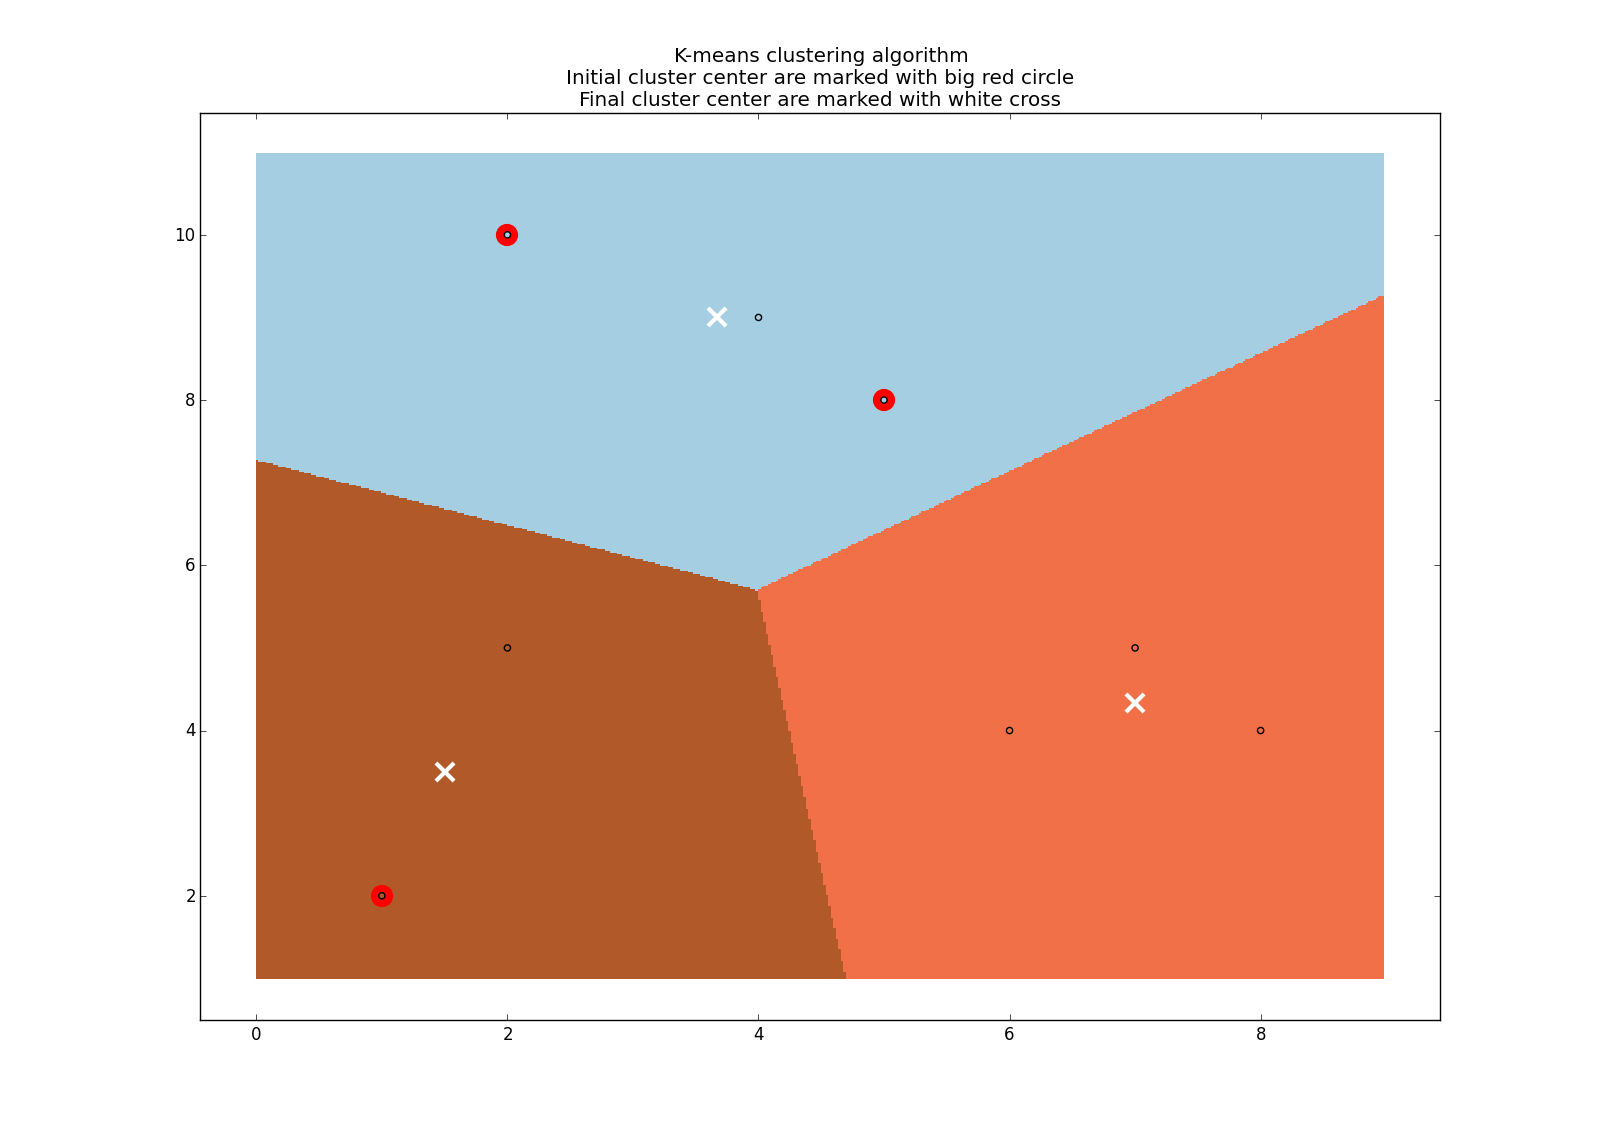
\includegraphics[scale=0.5]{3b.png}
\end{figure}

Das Ergebnis aus \nameref{subsec:kMeansClust} geht in die richtige Richtung, 
wenn die Iterationsanzahl in \nameref{subsec:kMeansClust} höher wäre, wäre das Ergebnis besser.
Der minimale Wert von \textit{max\_iter} ist $3$, wie in \autoref{fig:exercise3b} zu entnehmen ist.

,jedoch wird eine Iterationen mehr benötigt, um festzustellen, dass sich die Mittelwerte nicht ändern.

\subsection{c)}

\begin{figure}
\centering
\begin{subfigure}[b]{\linewidth}
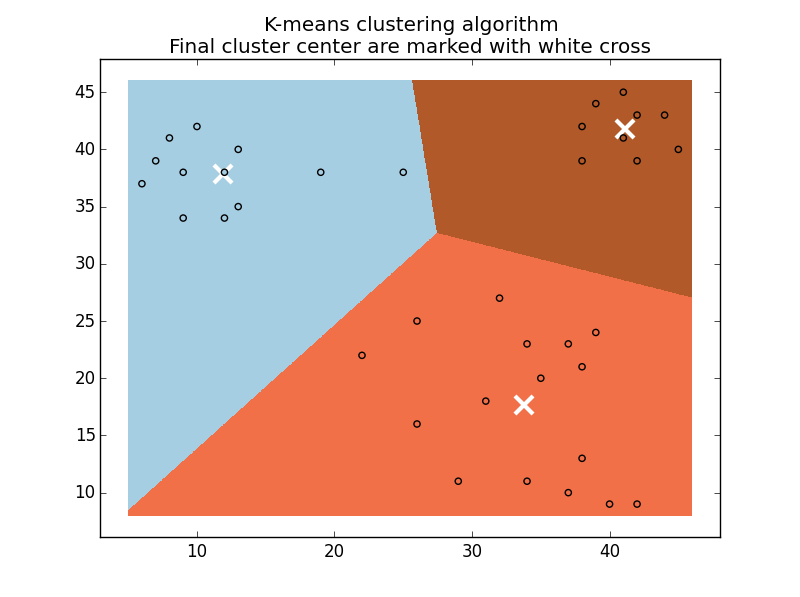
\includegraphics[scale=0.5]{3cRND1}
\end{subfigure}
\qquad
\begin{subfigure}[b]{\linewidth}
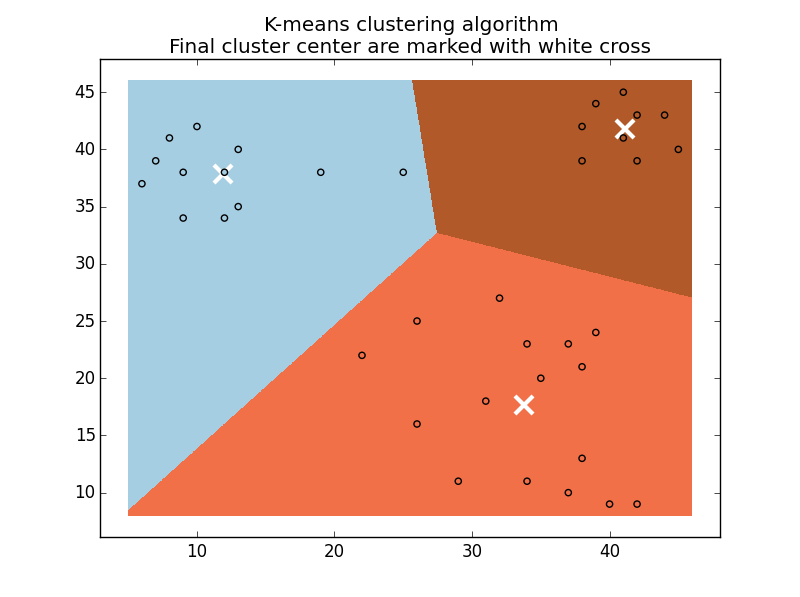
\includegraphics[scale=0.5]{3cRND2}
\end{subfigure} \\
\begin{subfigure}[b]{\linewidth}
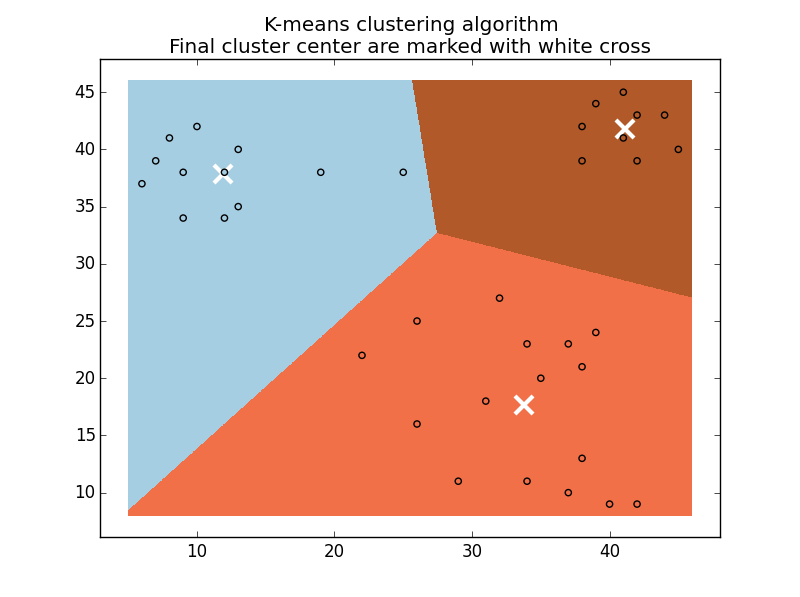
\includegraphics[scale=0.5]{3cRND3}
\end{subfigure}
\qquad
\begin{subfigure}[b]{\linewidth}
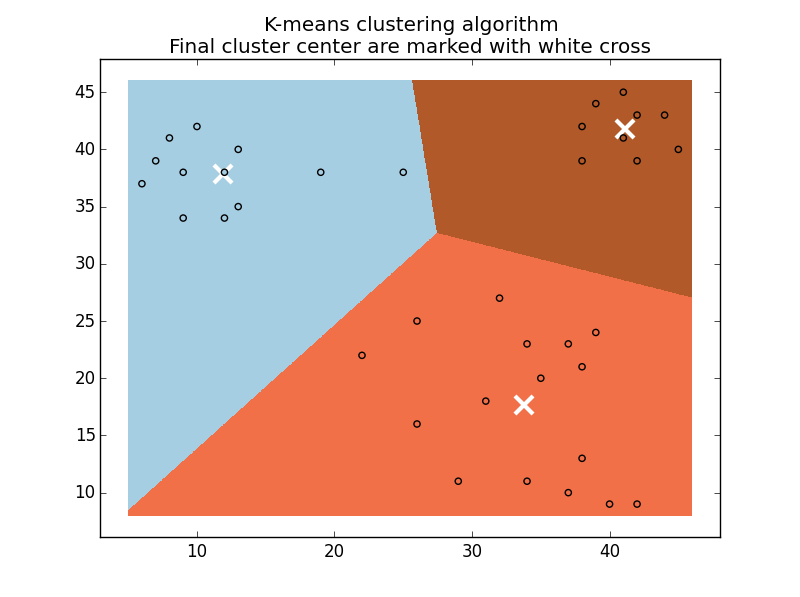
\includegraphics[scale=0.5]{3cRND4}
\end{subfigure}
\caption{4 Bildchen}
\end{figure}


\end{document}